\subsection{Antal pol/nulpunkt par}
\label{AntalPol_Nulpunktpar}
%
Et pol/nulpunkt par angiver at, der er et RC-led i tilbagekoblingen. Et RC-led består af en modstand i serie med en kondensator, hvor modstanden sørger for at forstærkningen er korrekt og kondensatoren sørger for knækfrekvensen, hvor hældningen begynder at falde.
Inden det afgøres hvor mange pol/nulpunkt par der skal anvendes, er det nødvendigt at omregne forstærkningen i dB, $G_{0(dB)}$, til en råforstærkning $G_0$:
%
\begin{equation}
	20*log_{10}(G_0) = G_{0(dB)} = 2.62dB
\end{equation}
%
Derfra isoleres $G_0$:
%
\begin{equation}
	G_0 = 10^{\frac{G_{0(dB)}}{20}} = 10^{\frac{2.62dB}{20}} = 1.3521
	\label{equ:Gain}
\end{equation}
%
For at få en indikation af hvor mange pol/nulpunkt par, svarende til antallet af RC-led, der skal anvendes udarbejdes \autoref{fig:1-8RC-ledIkkeJusteretC}.
%
\begin{figure}[H]
	\centering
	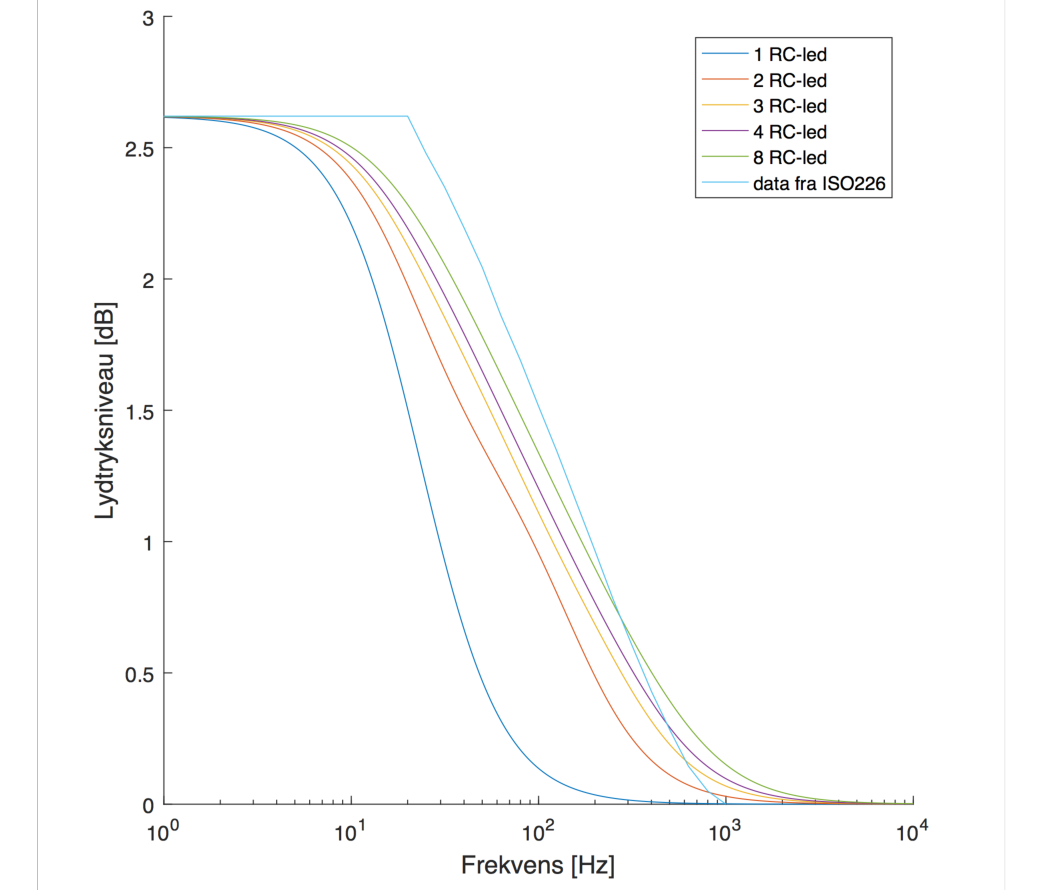
\includegraphics[resolution=300,width=\textwidth]{Figure/DesignAfFilter/1,2,3,4,8RC-ledGain2,62SHORT.pdf}
	\caption{Hældning per dekade for henholdsvis 1, 2, 3, 4 og 8 RC-led, hvor den logaritmiske x-akse angiver frekvens i hertz og den lineære y-akse angiver lydtryksniveau i dB.}
	\label{fig:1-8RC-ledIkkeJusteretC}
\end{figure}
\noindent
%
Kurven for $data fra ISO226$, på \autoref{fig:1-8RC-ledIkkeJusteretC}, repræsenterer resultatet af den teoretisk bedste overføringsfunktion, hvor knækket er ved præcis 20Hz, hvorfor der intet indrulningsforløb er, og hældningen er lineær mellem 20Hz og 1000Hz. RC-ledende er beregnet ud fra en forstærkning på 2.62dB, og samtlige udregninger er vedlagt i \autoref{app:Beregninger af RC-led}. Ydermere er polen valgt ved 20Hz, hvorfra kondensatorværdien udregnes:
%
\begin{equation}
	\omega_z = \frac{1}{R*C}		
\end{equation}  
%
Hvor nulpunktet $\omega_z$ er:
%
\begin{equation}
	\omega_z = 2*\pi*f 
\end{equation}
%
Isoleres kondensatoren, $C$, fåes følgende udtryk:
%
\begin{equation}
	C = \frac{1}{R*\omega_z} = \frac{1}{R*2*\pi*f}
\end{equation} 
%
Beregningerne for de RC-led der repræsenteres på \autoref{fig:1-8RC-ledIkkeJusteretC} fremgår i \autoref{app:Beregninger af RC-led}, og vil derfor ikke blive inkluderet her. Målet er at vælge det antal pol/nulpunkt par, antal RC-led, som sikre linearitet mellem 20Hz og 1000Hz, under den forudsætning at ved 20Hz skal der være en forstærkning på 2.62dB og ved 1000Hz skal der være en forstærkning på 0dB. På baggrund af det fravælges et RC-led, da hældningen er for stejl og der er ingen mulighed for at ændre på hældningen, da pol/nulpunkt parret kun har en effekt på x-aksen. 

Endvidere fravælges det at arbejde med to RC-led, da det ikke opnår en ren linearitet mellem 20Hz og 1000Hz, som det fremgår på \autoref{fig:1-8RC-ledIkkeJusteretC} er der et mindre knæk på kurven. Derimod hvis der arbejdes med tre RC-led opnåes et næsten fuldkomment lineært forløb mellem 20Hz og 1000Hz, jævnfør \autoref{fig:1-8RC-ledIkkeJusteretC}, dog forekommer der både et indrulnings- og udrulningsforløb, som skal justeres for at målet kan opfyldes. Da målet om linearitet mellem 20Hz og 1000Hz ikke forbedres ved at vælge fire eller otte RC-led, fravælges disse og der arbejdes derfor kun med tre RC-led.

På baggrund af det bliver hvert af de fire fraktal ordens filte, som skal sørger for at forstærkningen af de lave frekvenser foregår i overensstemmelse med forstærkningen fremsat i \autoref{tab:ForstaerkningTilDeSyvFiltre}, designet med  tre pol/nulpunkt par, og dermed tre RC-led.
%
\newpage
\noindent
% 